\documentclass[12pt]{article}
%\usepackage[margin=1in]{geometry} 
\usepackage{geometry}
\geometry{
	a4paper,
	total={150mm,257mm}
}
\usepackage{amsmath,amsthm,amssymb,amsfonts,listings,graphicx,caption,subcaption,hyperref}

\begin{document}
	\title{House Prices Analysis with Regression}
	\author{Pengshuai Shi}
	\maketitle
	
\section{Introduction}
For home buyers who just started looking into houses, they probably would not begin with asking for \textit{BsmtQual}(the height of the basement), number of fireplaces or \textit{MasVnrType}(Masonry veneer type) in the right beginning, but by visualizing and analyzing a housing price data set with regression, we will see how each of those attributes of a house could influence its sale price.
\section{Data Source}
The \textit{Ames Housing dataset}\footnote{\url{https://ww2.amstat.org/publications/jse/v19n3/decock.pdf}} compiled by Dean De Cock is a modernized and expanded alternative version of the often cited \textit{Boston Housing dataset}, it contains 80 columns in total, with 79 being the explanatory variables which includes many dfifferent aspects of an residential house such as \textit{LotArea, MSZoning, BsmtExposure} etc. in Ames, Iowa, and the last one is the sale price in dollars. 
\\
In this project, there are 1,460 data points in training set and 1,459 in testing set.
\section{Data-Preprocessing}
\subsection{Missing Data}
Before we proceed to analyze the data set using regression, we need to make sure it does not have missing values in the data set since regression model expects complete attribute from data. A quick search query shows that there are 1,460 number of rows each contains at least one missing value. Simple deletion would not work here as it would just remove our whole data set. So let us take a look of what attributes are missing and how many are missing in each attribute \ref{fig:sub1},\\
\\
It is also possible that test set could have missing values in an attribute that does not have missing data in training set, therefore we should also check \ref{fig:sub2},\\
\begin{figure}
	\centering
	\begin{subfigure}{.5\textwidth}
		\centering
		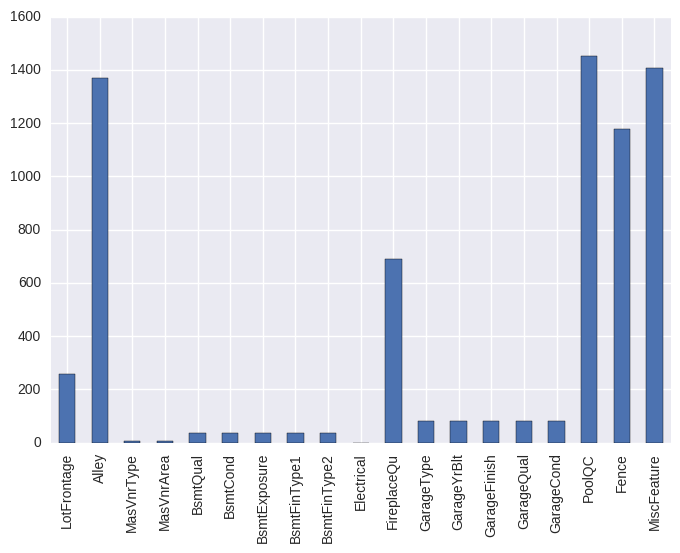
\includegraphics[width=\linewidth]{train_miss.png}
		\caption{train}
		\label{fig:sub1}
	\end{subfigure}%
	\begin{subfigure}{.5\textwidth}
		\centering
		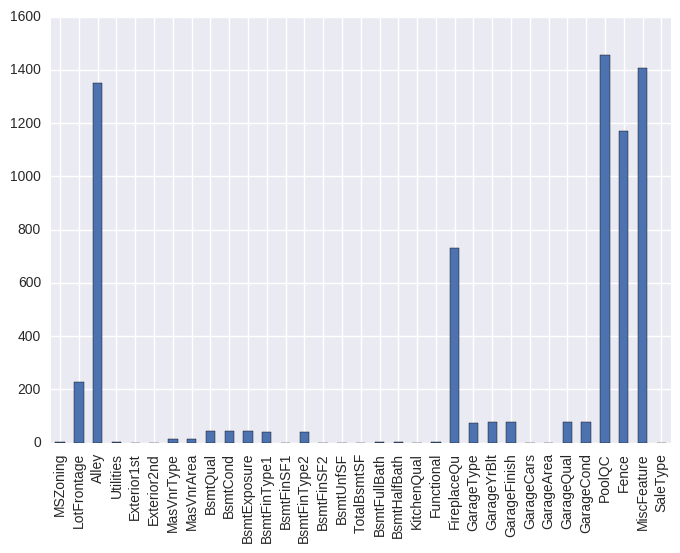
\includegraphics[width=\linewidth]{test_miss.png}
		\caption{test}
		\label{fig:sub2}
	\end{subfigure}
	\caption{Numer of missing data points}
\end{figure}\\
Thus we can see that both train and test set has 6 attributes with more than 15\% missing, and these six features is discarded - \textit{Fence, LotFrontage, MiscFeature, Alley, FireplaceQu, PoolQC}.\\
\\
A simple imputation method - replace missing points with mean or median of each column,  is used to fill up missing data points in the rest of attributes, although more sophiscated method can be used e.g. MICE(multiple imputation through chained equation), but the end result does not differ by much.
\subsection{Outliers}
It might also be helpful to look at some attributes and see if there is outliers, this is more relative to the model we are using. The objective function or the loss, which linear regression is trying to minize is very sensitive to outliers(absolute loss is less sensitive comparing to square loss),
\begin{figure}[h!]
	\centering
	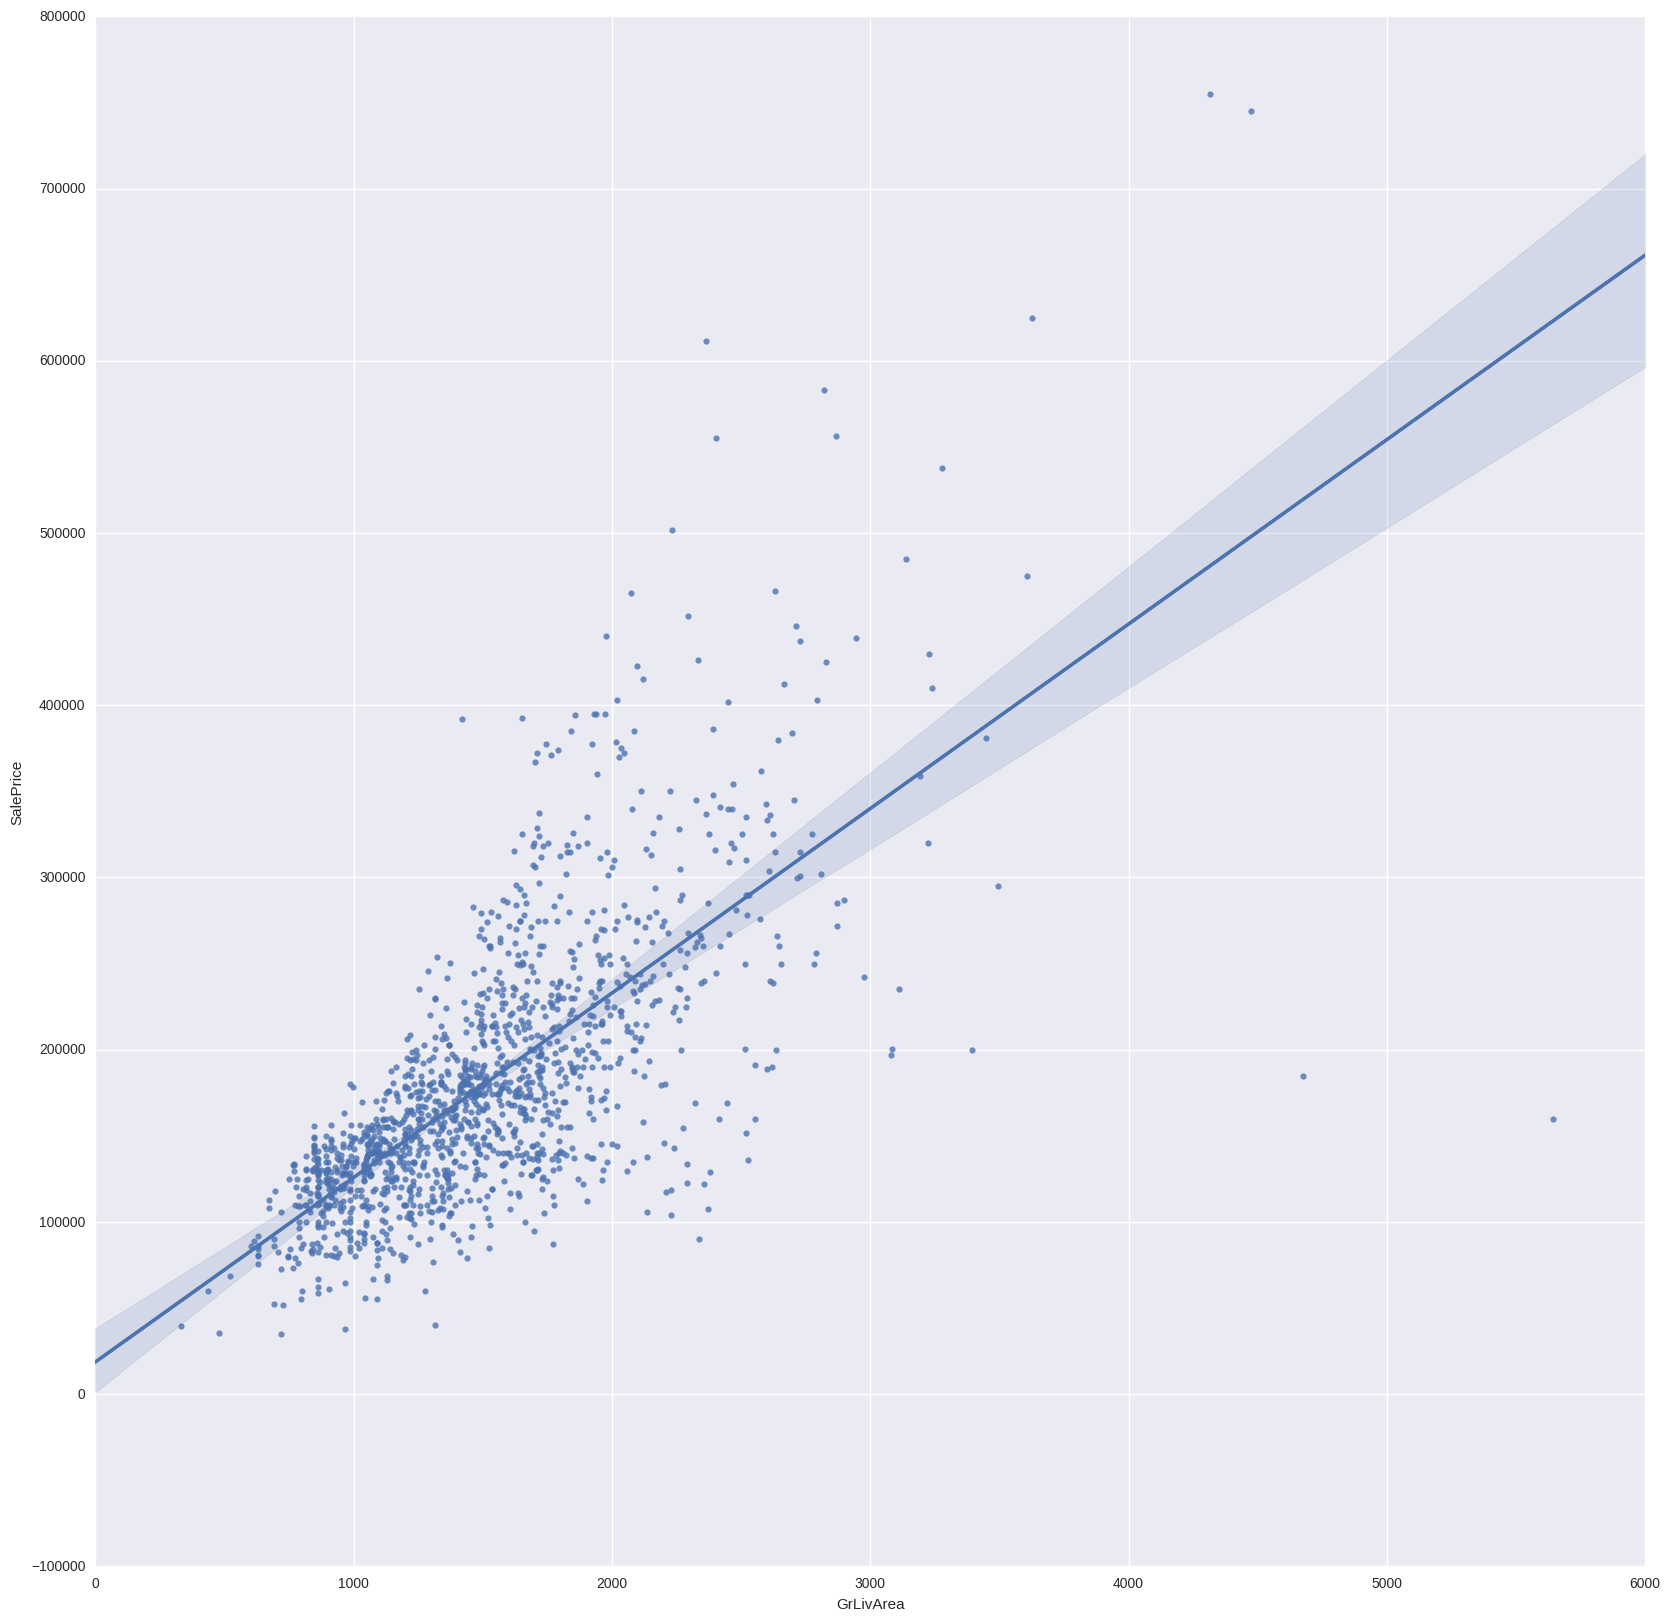
\includegraphics[width=0.6\linewidth]{outlier.png}
	\caption{Outliers in GrLiveArea}
	\label{fig:1}
\end{figure}
We can clearly see at the bottom right corner there are two data points that are likely to be outliers. In general, we want to remove it and see how the model perform, possible reasons we might not want to remove are that: in one dimension(GrLiveArea) they might appear to be away from main stream but it is not the case when we consider the complete feature space, and we may end up overfitting our train set. Nevertheless, they are removed in this project and we do observe a better performance overall, see the plot of all attributes in Fig \ref{fig:A} Appendix A. 
\subsection{Skewness}
First examine the distribution of the y-value \textit{SalePrice}, 
\begin{figure}[h!]
	\centering
	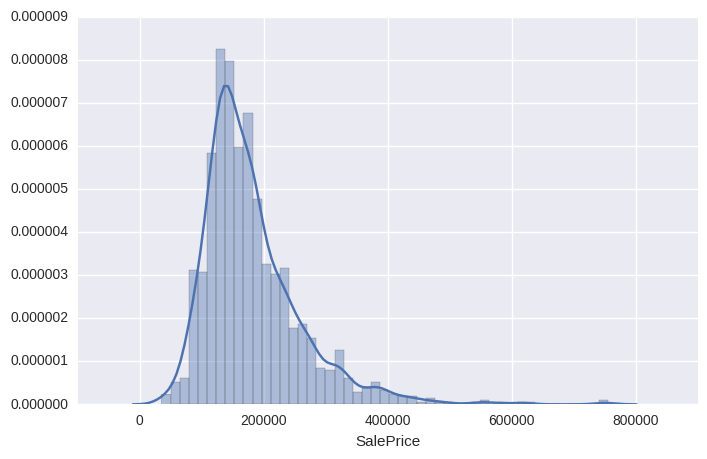
\includegraphics[width=0.6\linewidth]{skew.png}
	\caption{Histogram of SalePrice}
	\label{fig:2}
\end{figure}
so we see that the distribution of y-value is right-skewed, we apply \textit{log1p} transformation on SalePrice, i.e. $\log(\text{SalePrice} + 1)$, below is the result of the transformation,
\begin{figure}[h!]
	\centering
	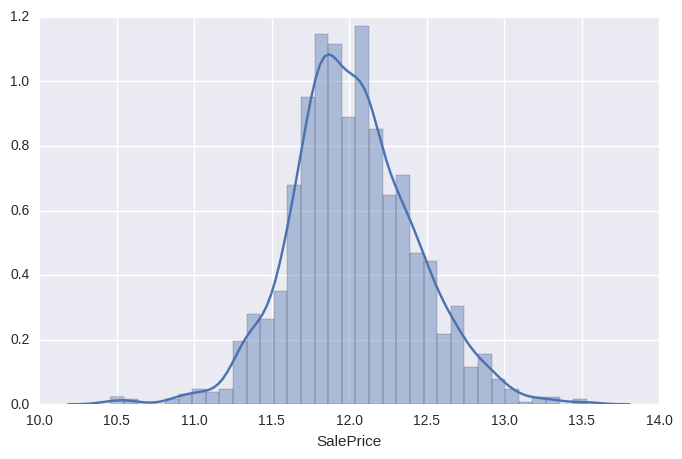
\includegraphics[width=0.6\linewidth]{skew_after.png}
	\caption{Histogram of SalePrice After \textit{log1p} Transformation}
	\label{fig:3}
\end{figure}
this might help our regression (it would not help, for example, tree models) and we apply this transformation to all skewed attributers, see Fig \ref{fig:B} in Appendix B.
\subsection{Multicollinearity}
Multicollinearity is where two or more features in a regression model being highly correlated, it can make our conclusions from regression less reliable, produce worse result and limit our conclusions.\\
\\
So we also want to check multicollineary in our attributes, below is a table of correlation between a pair of features in descending order, 
\begin{verbatim}
 	  cor 	     pair
 	 	0.887304 	(GarageArea, GarageCars)
 	 	0.853926 	(Exterior2nd, Exterior1st)
 	 	0.851185 	(BsmtFinSF2, BsmtFinType2)
 	 	0.822983 	(TotRmsAbvGrd, GrLivArea)
 	 	0.794597 	(YearBuilt, GarageYrBlt)
 	 	0.783890 	(1stFlrSF, TotalBsmtSF)
 	 	0.780687 	(BsmtFinSF1, BsmtFinType1)
 	 	0.680390 	(TotRmsAbvGrd, BedroomAbvGr)
 	 	0.652879 	(GrLivArea, FullBath)
 	 	0.636755 	(ExterQual, KitchenQual)
\end{verbatim}
\begin{figure}[h!]
	\centering
	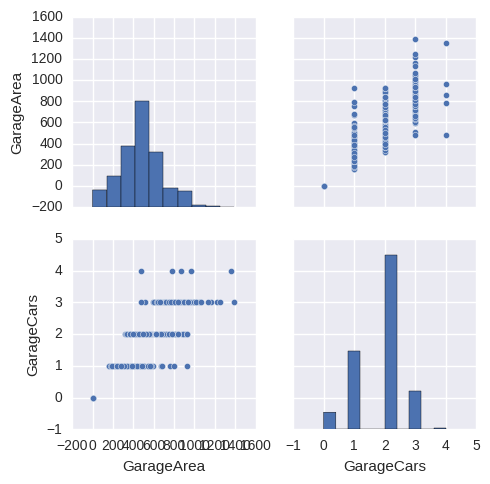
\includegraphics[width=0.6\linewidth]{cor.png}
	\caption{Correlation between GarageArea and GarageCars}
	\label{fig:4}
\end{figure}
The plot is reasonable since in general the number of cars one can park in the garage is highly positive correlated with the garage area. Then we only need to choose one of the two features for regression model.
\subsection{Standardization}
Substract mean of each column on each data point and division by the standard deviation is applied to train and test data set. The reason we should perform standardization is that, regression is also sensitive to the scales differernce between our features. \\
\\
For example, \textit{years} and \textit{area}, the former is on the scale around 2,000 but the latter one might around 0.5 scale. This difference would overshadow the effect of \textit{area} in the regression model: $y = a_1\cdot\text{years}+a_2\cdot\text{area}+ ...$, and \textit{loss} = $\sum(y-y_{\text{pred}})^2$, the huge value in the square would cover up the value from \textit{area}. 
\section{Models}
\subsection{Lasso Regression}
Lasso regression is a type of regularized regression. The reason we choose it over ordinary linear regression and ridge regression is that, it is less likely to overfit and this is important in this project since the data set has a relatively large features space thus higher degree of freedom to overfit, the regularization term is less sensitive to outliers and it also comes with feature selection.\\
\\
This is the objective function Lasso is trying to minimize:
\begin{equation*}
\frac{1}{2n_{\text{sample}}}\sum_{i}^{n_{\text{sample}}}||y-x_i^Tw||^2 + \alpha\sum_{j}^{d_{\text{features}}}||w||_1
\end{equation*}
where $||w||_1$ is the $L_1$ norm.\\
The metric we use to evaluate our is $r^2$ - coefficient of determination,
\begin{equation*}
r_2=\frac{\text{explained variation}}{\text{total variation}}
\end{equation*}
it is a measure of how close the observed data to the fitted regression line. \\
\\
Linear\_model.Lasso\cite{lasso} from \textit{sklearn} is used to train our model on the 1,460 training set, procedure:
\begin{itemize}
\item Perfrom gridsearch by cross-validation\cite{gs} to find the best hyper-parameter, in this case - $\alpha$.\\
\\
The gridsearch\_cv is performed over 100 different values of $\alpha$ between 0 to 1, where 0 is same as ordinary least square regression, and value closer to 1 corresponds to higher penalty, below is the cross-validation $r2$ result over $\alpha$ in log scale:
\begin{figure}[h!]
	\centering
	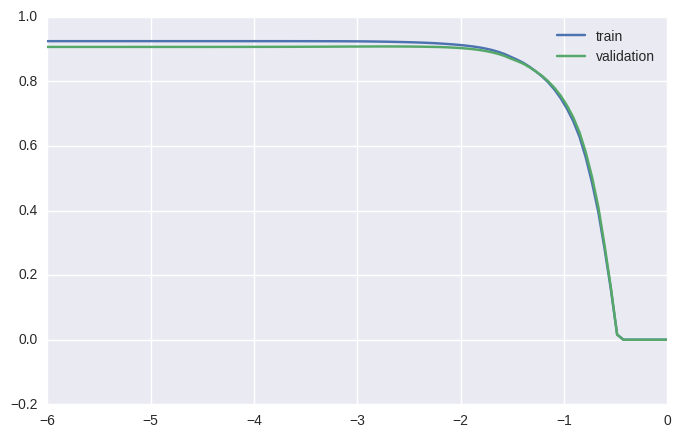
\includegraphics[width=0.65\linewidth]{alpha.png}
	\caption{Grid search through cross-validation over $\alpha$}
	\label{fig:5}
\end{figure}\\
the best result and parameter is: $r_2=0.91078$ and $\alpha=0.0014$.\\
\\
Lasso also produces feature importance, i.e. based on the magnitude of coefficient of each feature we can tell which feature is more important to the model:
\begin{figure}[h!]
	\centering
	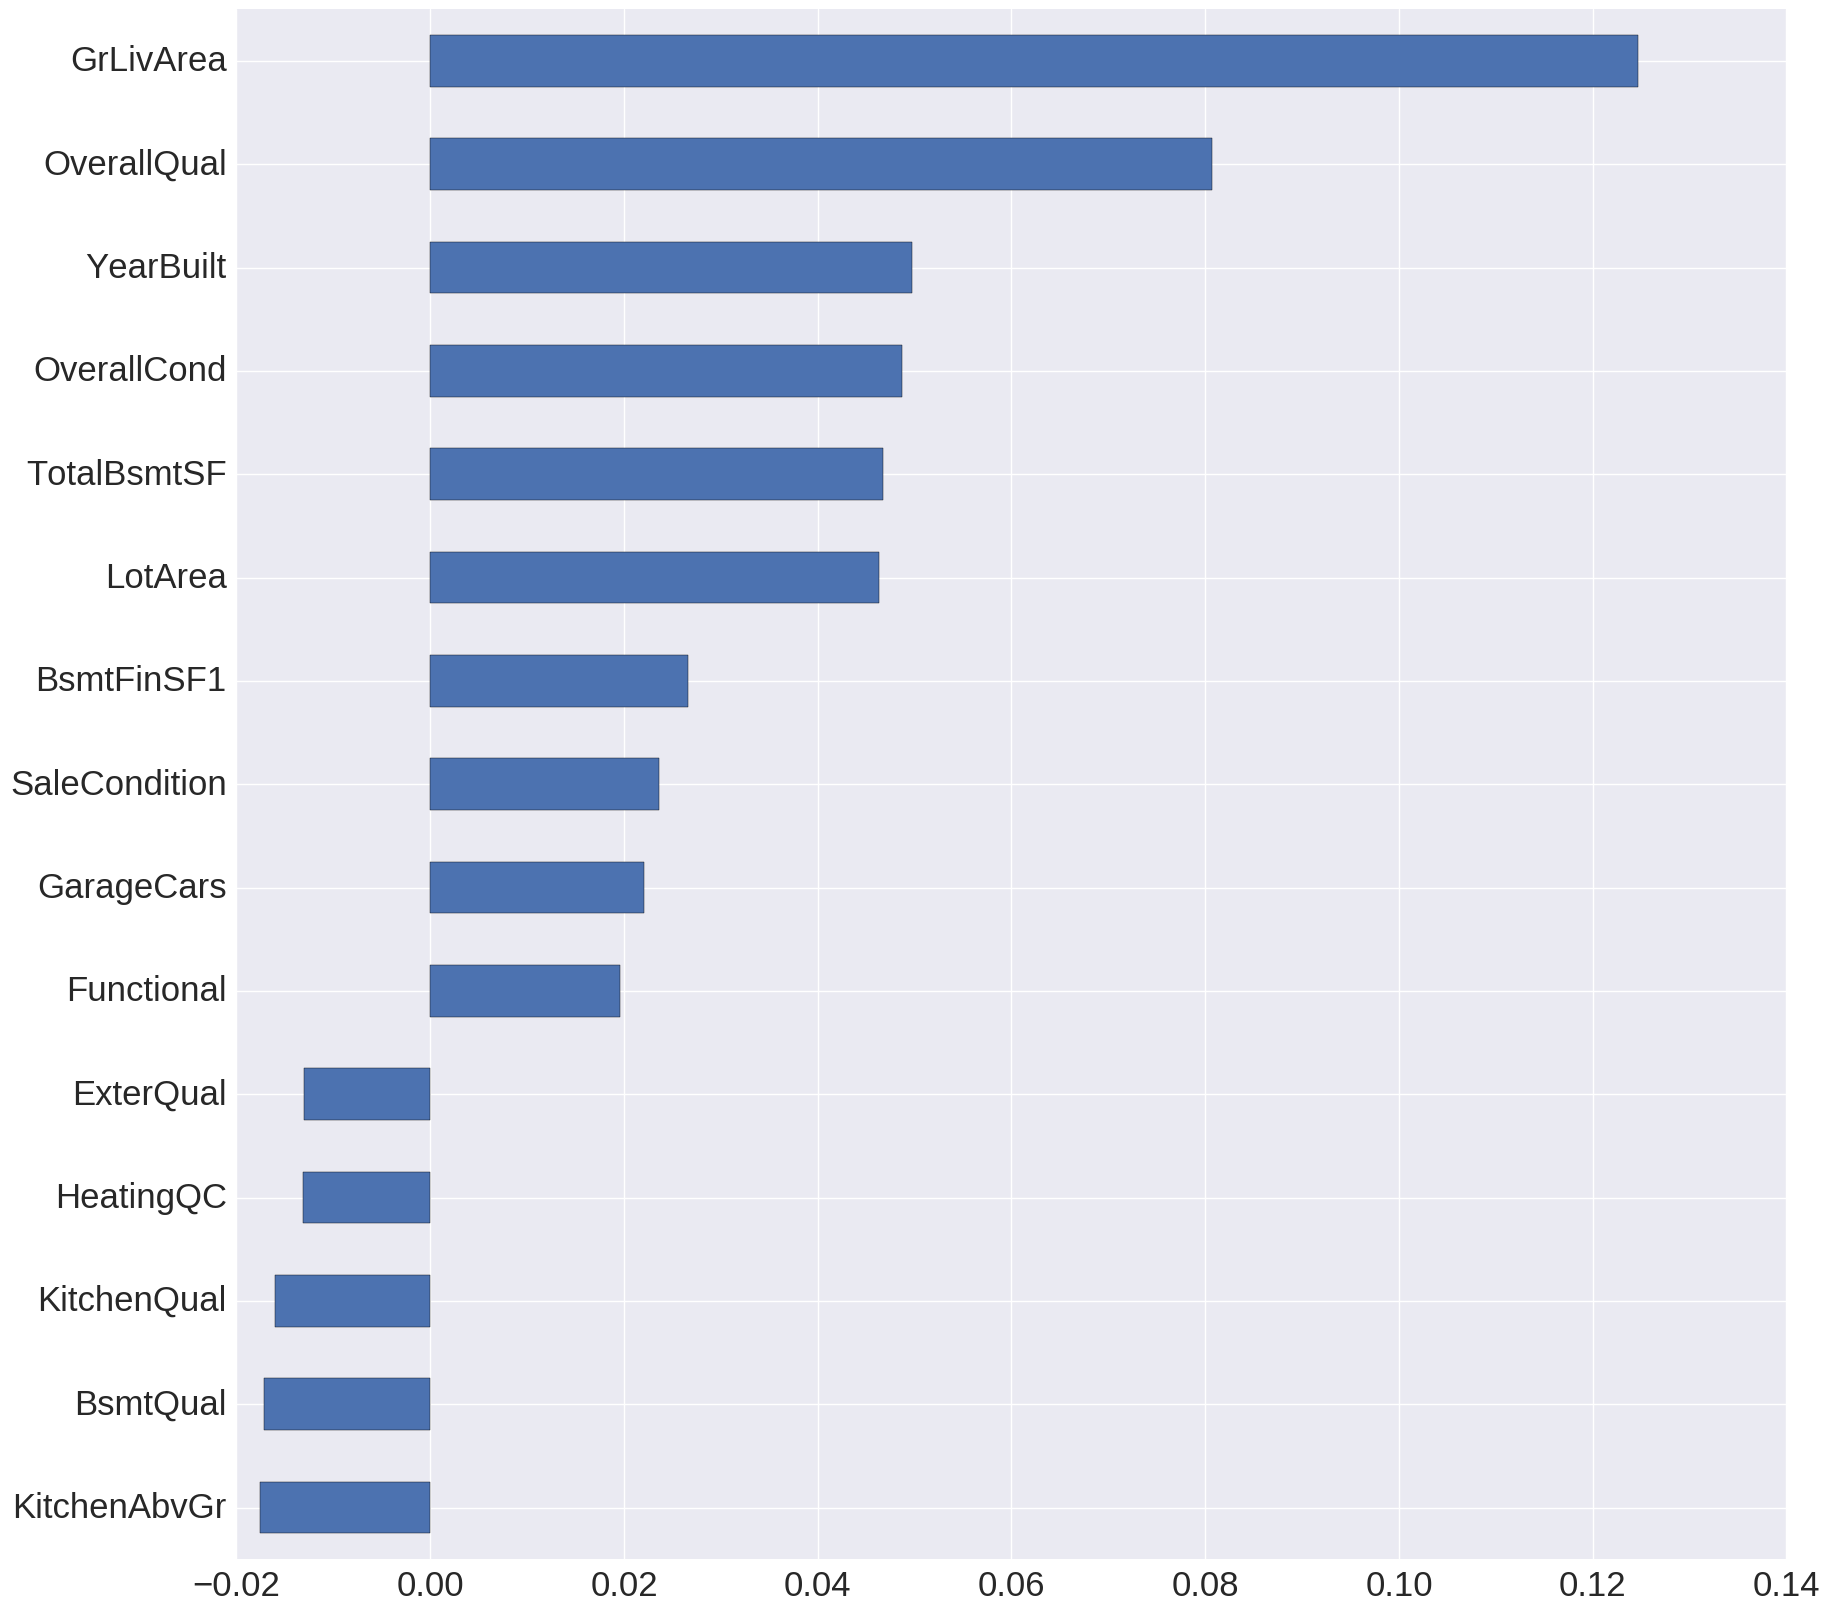
\includegraphics[width=0.8\linewidth]{fts_imp.png}
	\caption{Feature importance}
	\label{fig:6}
\end{figure}
\\
from this we can conclude that, 
\begin{itemize}
\item GrLivArea: Above grade (ground) living area square feet
\item OverallQual: Overall material and finish quality
\item YearBuilt: Original construction date
\item OverallCond: Overall condition rating
\item TotalBsmtSF: Total square feet of basement area
\item LotArea: Lot size in square feet
\end{itemize}
are the top 6 most important features in deciding the \textit{SalePrice} of the house.
\item Make predictions on test set, ensemble several predictions over different split of training data to make final prediction, below is the result of each run,
\begin{verbatim}
[CV 0]
r2: 0.927136691308
RMSLE: 0.119979309487
[CV 1]
r2: 0.92101279528
RMSLE: 0.109265058538
[CV 2]
r2: 0.920464664871
RMSLE: 0.110925238648
[CV 3]
r2: 0.927579929518
RMSLE: 0.124577910439
[CV 4]
r2: 0.916725315748
RMSLE: 0.122738038905
[CV 5]
r2: 0.921750128229
RMSLE: 0.125474602726
\end{verbatim}
where we also include a different evaluation metrics \textit{RMSLE} - root mean squared error in log scale, overall the results are consistent and produce good fit. 
\end{itemize}
\subsection{Gradient Boosting}
We would like to compare the result from Lasso regression with Gradient Boosting, \textit{gradient boosting} is a technique that fits an additive model in a forward stage-wise manner, in each stage a weak learner is introudced to compensate the shortcomings of previous learners, for example, we start with a base learner called $F(x)$, where it approximately predicts the correct $y$ value, 
\begin{equation*}
	F(x) \approx y
\end{equation*}
we hope to improve the model by adding a function $h(x)$ so that:
\begin{equation*}
F(x) + h(x) = y
\end{equation*}
then $h(x)$ can be learned through regression:
\begin{equation*}
h(x) = y-F(x)
\end{equation*}
if now the new model $F_1(x)=F(x)+h(x)$ still does not perform very well then we can repeat the addition until satisfied \cite{gb_explain}.\\
\\
ensemble.GradientBoostingRegressor\cite{gb} in \textit{sklearn} is used to build our model. Similar to the procedures in Lasso, we perform gridsearch\_cv to find the best set of parameters, and following is the best $r_2$ result and the best hyper-parameters:
\begin{verbatim}
r2 = 0.911430559844
{'max_features': 0.05, 'learning_rate': 0.01, 'max_depth': 3,
 'min_samples_leaf': 3}
\end{verbatim}
and we can also compare the important features produced by gradient boosting, see Fig\ref{fig:7}.\\
\begin{figure}[h!]
	\centering
	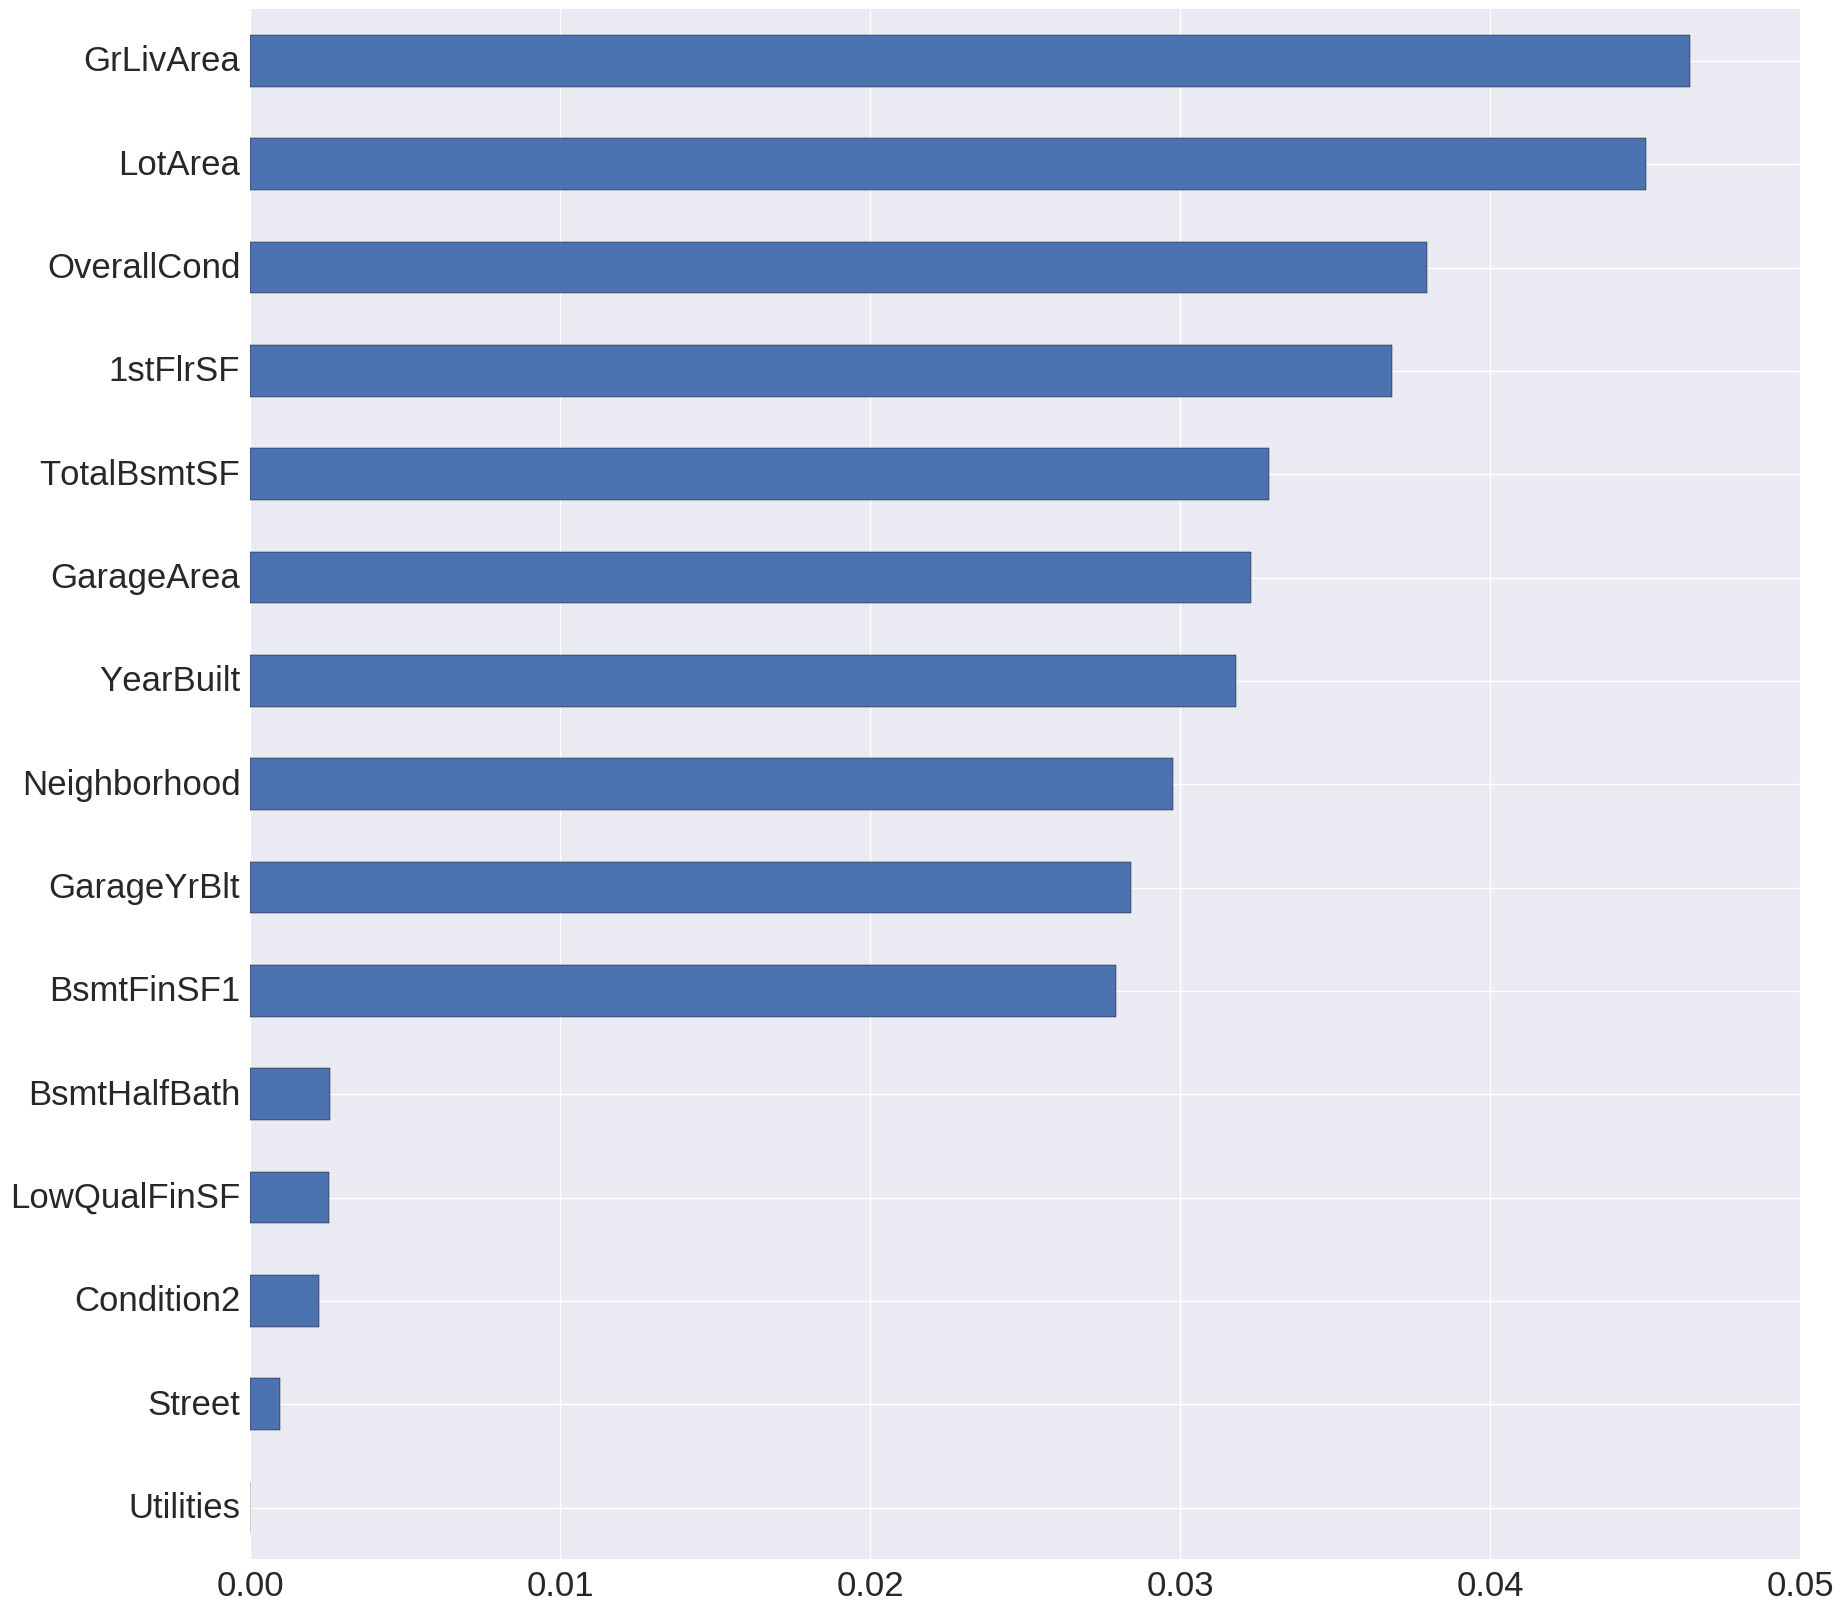
\includegraphics[width=0.8\linewidth]{gb_imp.png}
	\caption{Feature importance in gradient boosting}
	\label{fig:7}
\end{figure}
\\ Ensemble the result from model using different resampled data,
\begin{verbatim}
[CV 0]
r2: 0.936931009404
RMSLE: 0.11085110698
[CV 1]
r2: 0.925904712222
RMSLE: 0.104461990165
[CV 2]
r2: 0.926120655209
RMSLE: 0.106887159554
[CV 3]
r2: 0.940035505163
RMSLE: 0.10932094716
[CV 4]
r2: 0.90448611194
RMSLE: 0.126568657859
[CV 5]
r2: 0.922382972786
RMSLE: 0.123227873843
\end{verbatim}
we see that it some times performs better than Lasso but it is less stable, the reason might be the variance and bias trade-off.\\
\\
The top 6 most importrant features:
\begin{itemize}
\item GrLivArea: Above grade (ground) living area square feet
\item LotArea: Lot size in square feet
\item OverallCond: Overall condition rating
\item 1stFlrSF: First Floor square feet
\item TotalBsmtSF: Total square feet of basement area
\item GarageArea: Size of garage in square feet
\end{itemize}

\section{Conclusions}
This housing data set has 6 attributes with more than 15\% of missing values, so data imputation is performed. It also contains several right skewed attribute, e.g. \textit{SalePrice} and \textit{log1p} transformation is used to normalize the skewed distribution. Finally, \textit{Lasso regression} and \textit{Gradient boosting} are used to predict \textit{SalePrice} of housing training data. Both of them achieves a good fit to observed data, $r2$ of Lasso is 0.91078 and gradient boosting is 0.91143. They also produce similar top 6 important features to the model, with a few differences, such as \textit{1stFlrSF, GarageArea and YearBuilt}.

\begin{thebibliography}{9}
	\bibitem{lasso} 
\url{http://scikit-learn.org/stable/modules/generated/sklearn.linear_model.Lasso.html}
	
	\bibitem{gb} 
\url{http://scikit-learn.org/stable/modules/generated/sklearn.ensemble.GradientBoostingRegressor.html}
	
	\bibitem{gb_explain} 
\url{http://www.ccs.neu.edu/home/vip/teach/MLcourse/4_boosting/slides/gradient_boosting.pdf}

\bibitem{gs} 
\url{http://scikit-learn.org/stable/modules/generated/sklearn.model_selection.GridSearchCV.html}
\end{thebibliography}


\newpage
\section*{Appendix}
\subsection*{A}
\begin{figure}[h!]
	\centering
	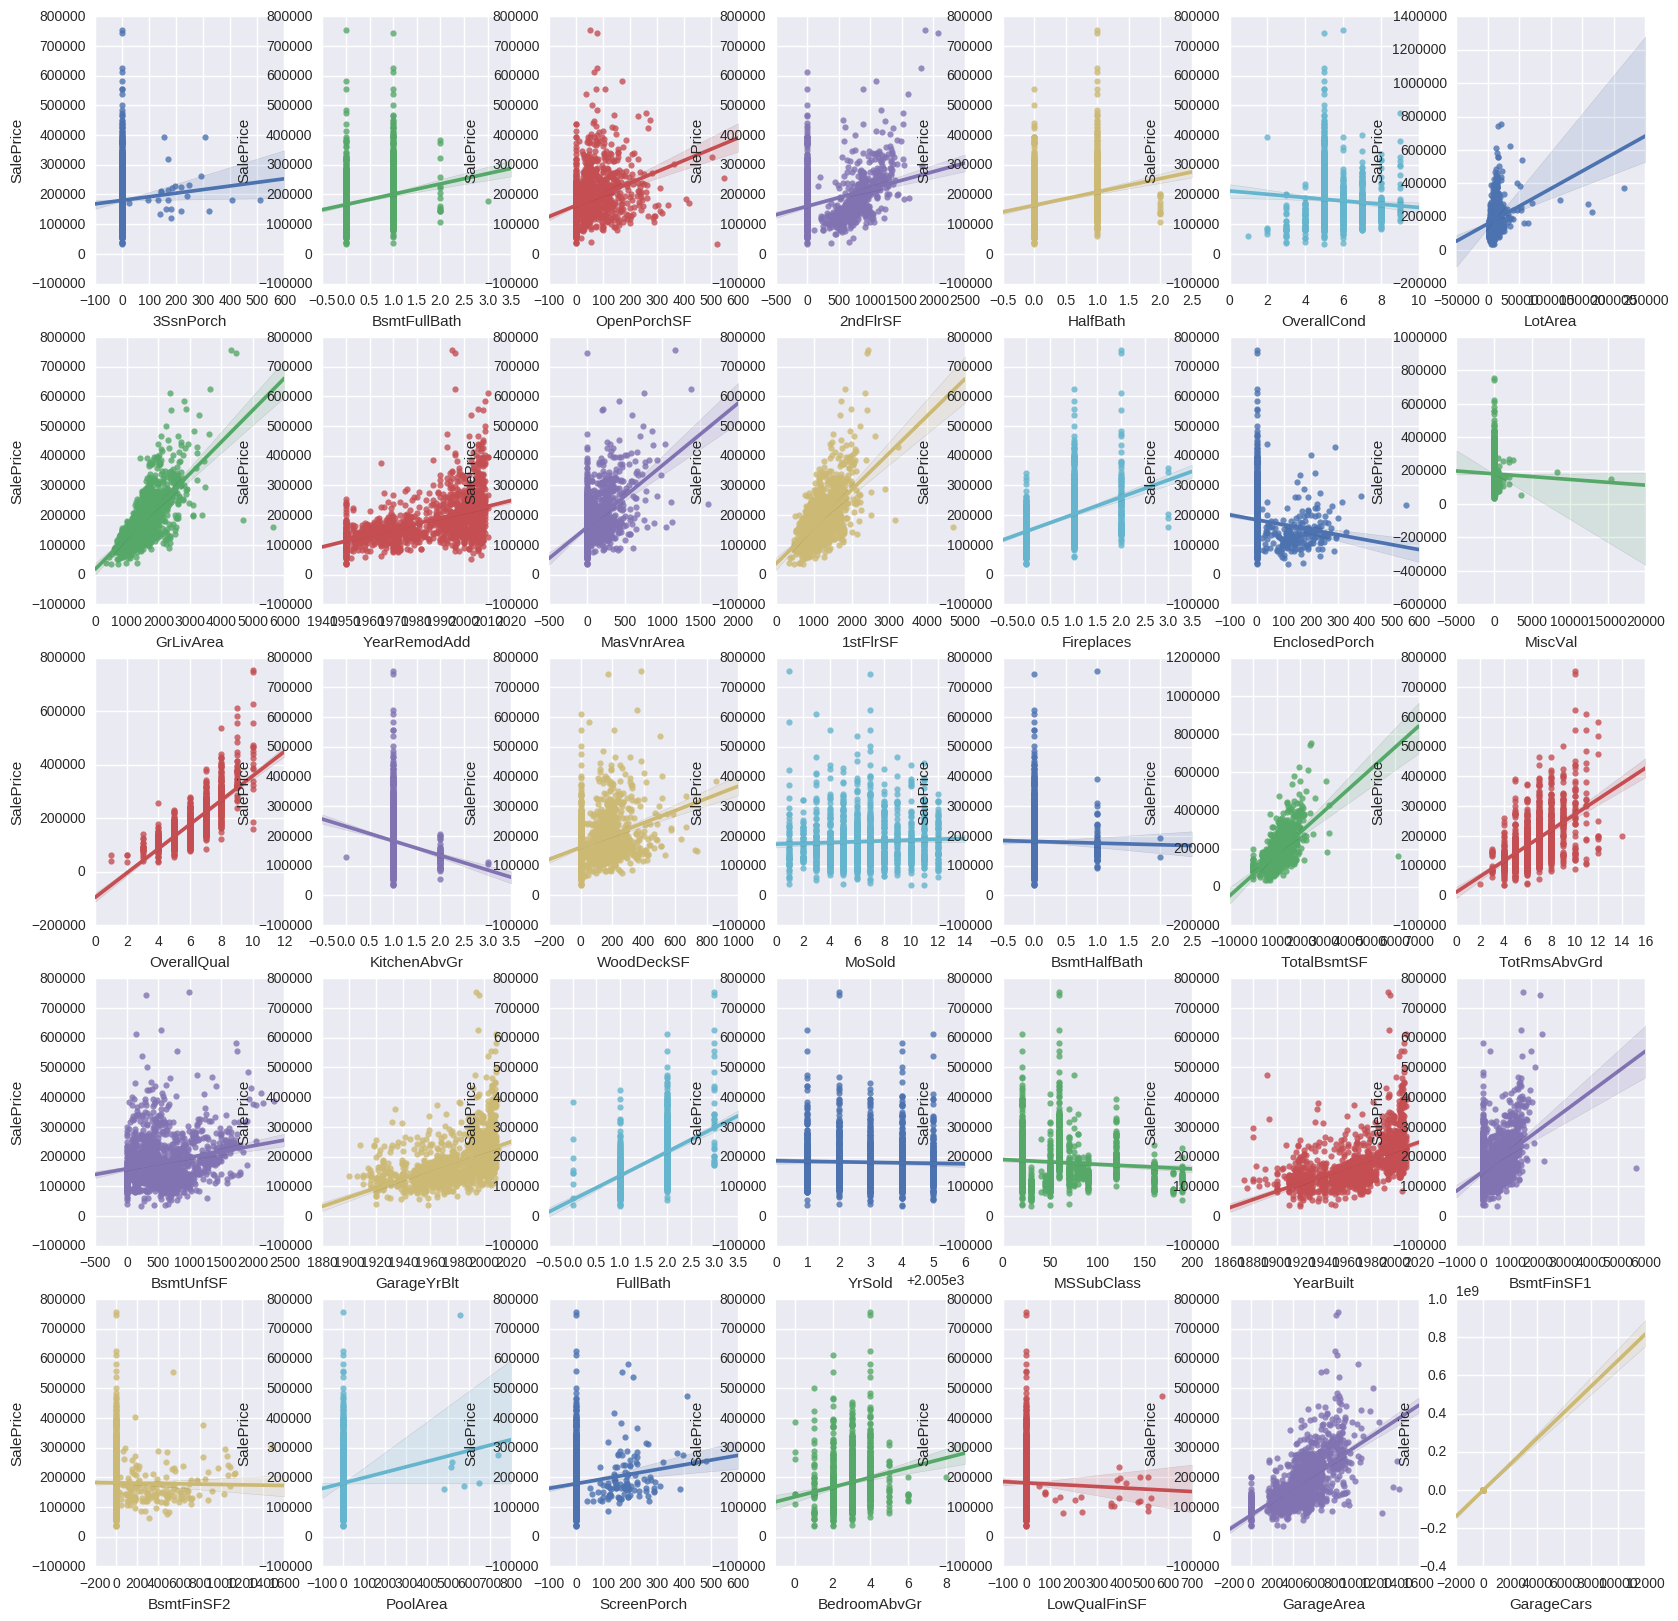
\includegraphics[width=\linewidth]{outliers_all.png}
	\caption{Attributes vs. SalePrice}
	\label{fig:A}
\end{figure}
\newpage
\subsection*{B}
\begin{figure}[h!]
	\centering
	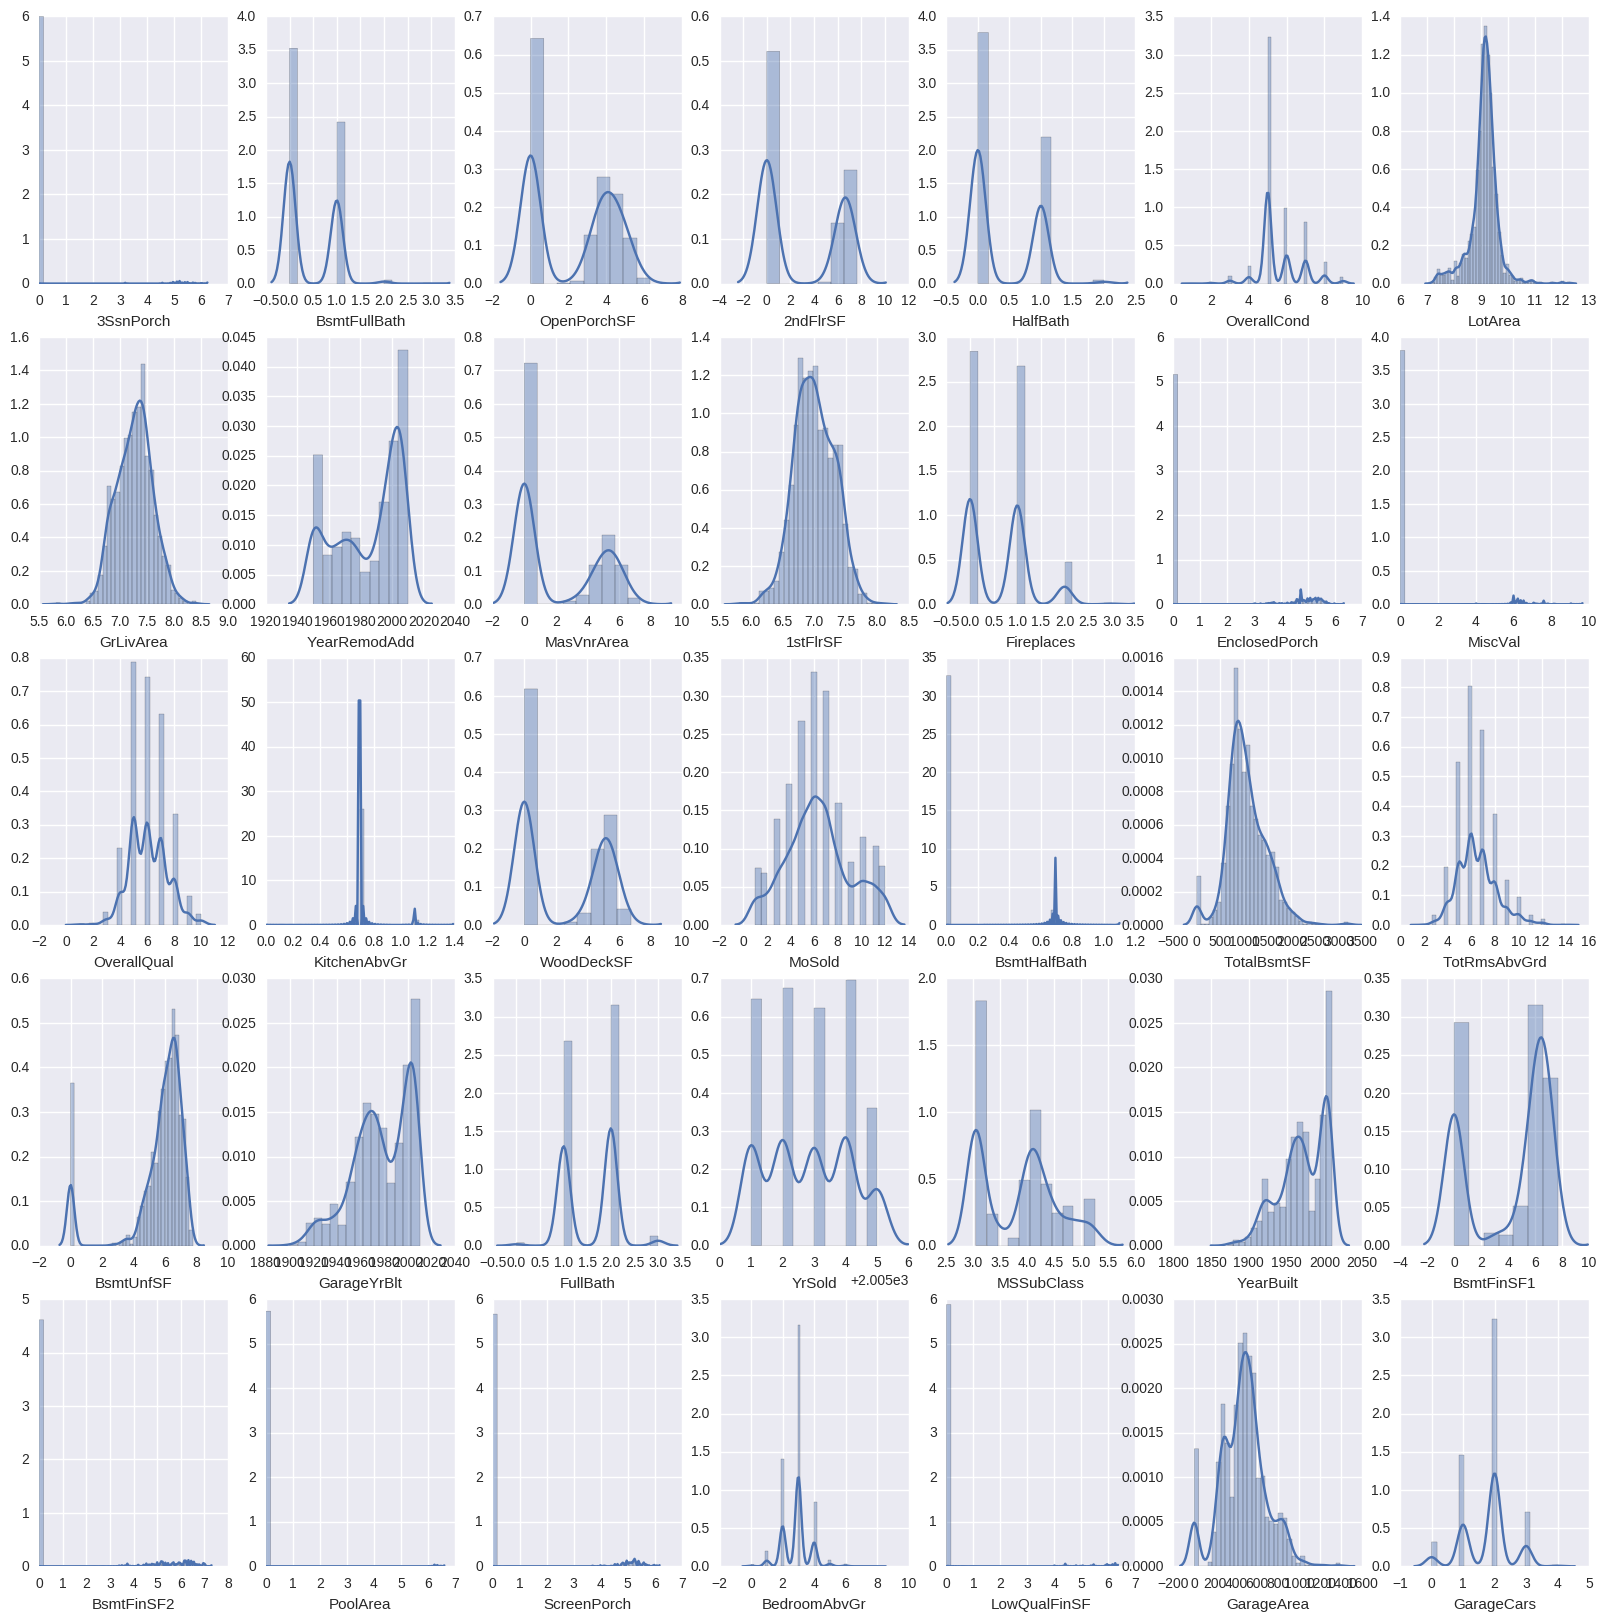
\includegraphics[width=\linewidth]{skew_all.png}
	\caption{Distribution After \textit{log1p} Transformation}
	\label{fig:B}
\end{figure}
\end{document}